\documentclass[12pt]{article}\usepackage[]{graphicx}\usepackage[]{color}
%% maxwidth is the original width if it is less than linewidth
%% otherwise use linewidth (to make sure the graphics do not exceed the margin)
\makeatletter
\def\maxwidth{ %
  \ifdim\Gin@nat@width>\linewidth
    \linewidth
  \else
    \Gin@nat@width
  \fi
}
\makeatother

\definecolor{fgcolor}{rgb}{0.345, 0.345, 0.345}
\newcommand{\hlnum}[1]{\textcolor[rgb]{0.686,0.059,0.569}{#1}}%
\newcommand{\hlstr}[1]{\textcolor[rgb]{0.192,0.494,0.8}{#1}}%
\newcommand{\hlcom}[1]{\textcolor[rgb]{0.678,0.584,0.686}{\textit{#1}}}%
\newcommand{\hlopt}[1]{\textcolor[rgb]{0,0,0}{#1}}%
\newcommand{\hlstd}[1]{\textcolor[rgb]{0.345,0.345,0.345}{#1}}%
\newcommand{\hlkwa}[1]{\textcolor[rgb]{0.161,0.373,0.58}{\textbf{#1}}}%
\newcommand{\hlkwb}[1]{\textcolor[rgb]{0.69,0.353,0.396}{#1}}%
\newcommand{\hlkwc}[1]{\textcolor[rgb]{0.333,0.667,0.333}{#1}}%
\newcommand{\hlkwd}[1]{\textcolor[rgb]{0.737,0.353,0.396}{\textbf{#1}}}%

\usepackage{framed}
\makeatletter
\newenvironment{kframe}{%
 \def\at@end@of@kframe{}%
 \ifinner\ifhmode%
  \def\at@end@of@kframe{\end{minipage}}%
  \begin{minipage}{\columnwidth}%
 \fi\fi%
 \def\FrameCommand##1{\hskip\@totalleftmargin \hskip-\fboxsep
 \colorbox{shadecolor}{##1}\hskip-\fboxsep
     % There is no \\@totalrightmargin, so:
     \hskip-\linewidth \hskip-\@totalleftmargin \hskip\columnwidth}%
 \MakeFramed {\advance\hsize-\width
   \@totalleftmargin\z@ \linewidth\hsize
   \@setminipage}}%
 {\par\unskip\endMakeFramed%
 \at@end@of@kframe}
\makeatother

\definecolor{shadecolor}{rgb}{.97, .97, .97}
\definecolor{messagecolor}{rgb}{0, 0, 0}
\definecolor{warningcolor}{rgb}{1, 0, 1}
\definecolor{errorcolor}{rgb}{1, 0, 0}
\newenvironment{knitrout}{}{} % an empty environment to be redefined in TeX

\usepackage{alltt}
\usepackage[english]{babel}
\usepackage[utf8x]{inputenc}
\usepackage{amsmath}
\usepackage{graphicx}
\usepackage[colorinlistoftodos]{todonotes}
\usepackage{xcolor}
\usepackage{framed}
\usepackage{tikz}
\usepackage{titletoc}
\usepackage{etoolbox}
\usepackage{lmodern}
\usepackage{hyperref}
\usepackage{verbatimbox}

% definition of some personal colors
\definecolor{myred}{RGB}{125,17,12}
\definecolor{myyellow}{RGB}{225,216,183}

% command for the circle for the number of part entries
\newcommand\Circle[1]{\tikz[overlay,remember picture] 
  \node[draw,circle, text width=18pt,line width=1pt] {#1};}

% patching of \tableofcontents to use sans serif font for the tile
\patchcmd{\tableofcontents}{\contentsname}{\sffamily\contentsname}{}{}
% patching of \@part to typeset the part number inside a framed box in its own line
% and to add color
\makeatletter
\patchcmd{\@part}
  {\addcontentsline{toc}{part}{\thepart\hspace{1em}#1}}
  {\addtocontents{toc}{\protect\addvspace{20pt}}
    \addcontentsline{toc}{part}{\huge{\protect\color{myyellow}%
      \setlength\fboxrule{2pt}\protect\Circle{%
        \hfil\thepart\hfil%
      }%
    }\\[2ex]\color{myred}\sffamily#1}}{}{}

%\patchcmd{\@part}
%  {\addcontentsline{toc}{part}{\thepart\hspace{1em}#1}}
%  {\addtocontents{toc}{\protect\addvspace{20pt}}
%    \addcontentsline{toc}{part}{\huge{\protect\color{myyellow}%
%      \setlength\fboxrule{2pt}\protect\fbox{\protect\parbox[c][1em][c]{1.5em}{%
%        \hfil\thepart\hfil%
%      }}%
%    }\\[2ex]\color{myred}\sffamily#1}}{}{}
\makeatother

% this is the environment used to typeset the section entries in the ToC
% it is a modification of the leftbar environment of the framed package
\renewenvironment{leftbar}
  {\def\FrameCommand{\hspace{6em}%
    {\color{myyellow}\vrule width 2pt depth 6pt}\hspace{1em}}%
    \MakeFramed{\parshape 1 0cm \dimexpr\textwidth-6em\relax\FrameRestore}\vskip2pt%
  }
 {\endMakeFramed}

% using titletoc we redefine the ToC entries for parts, chapters, sections, and subsections
\titlecontents{part}
  [0em]{\centering}
  {\contentslabel}
  {}{}
\titlecontents{section}
  [0em]{\vspace*{1.2\baselineskip}}
  {\parbox{4.5em}{%
    \hfill\Huge\sffamily\bfseries\color{myred}\thecontentspage}%
   \vspace*{-2.3\baselineskip}\leftbar\textsc{\small\thecontentslabel}\\\sffamily}
  {}{\endleftbar}
\titlecontents{subsection}
  [8.4em]
  {\sffamily\contentslabel{3em}}{}{}
  {\hspace{1.5em}\nobreak\itshape\color{myred}\contentspage}

\renewenvironment{abstract}
 {\small
  \begin{center}
  \bfseries \abstractname\vspace{-.5em}\vspace{0pt}
  \end{center}
  \list{}{
    \setlength{\leftmargin}{.5cm}%
    \setlength{\rightmargin}{\leftmargin}%
  }%
  \item\relax}
 {\endlist}
\IfFileExists{upquote.sty}{\usepackage{upquote}}{}
\begin{document}

\begin{titlepage}

\newcommand{\HRule}{\rule{\linewidth}{0.5mm}}

\center 
 
%----------------------------------------------------------------------------------------
%   HEADING SECTIONS
%----------------------------------------------------------------------------------------

\textsc{\LARGE Indiana University Bloomington}\\[1.5cm] 
\textsc{\Large CSCI B 565}\\[0.5cm] 
\textsc{\large Data Mining}\\[0.5cm] 

%----------------------------------------------------------------------------------------
%   TITLE SECTION
%----------------------------------------------------------------------------------------

\HRule \\[0.4cm]
{ \huge \bfseries Data Analytics for IU Bus System}\\[0.4cm] 
\HRule \\[1.5cm]
\large Group Name : RedMiners \\
 
%----------------------------------------------------------------------------------------
%   AUTHOR SECTION
%----------------------------------------------------------------------------------------

\begin{minipage}{0.4\textwidth}
\begin{flushleft} \large
\emph{Authors:}\\
\textsc{Jayasankar, Siddharth \ Nagarajan, Ganesh \ Madhavan, Sarvothaman } 
\end{flushleft}
\end{minipage}
~
\begin{minipage}{0.4\textwidth}
\begin{flushright} \large
\emph{Supervisor:} \\
\textsc{Dr. Dalkilic, Mehmet} 
\end{flushright}
\end{minipage}\\[2cm]


%----------------------------------------------------------------------------------------
%   DATE SECTION
%----------------------------------------------------------------------------------------

{\large \today}\\[2cm] 
%----------------------------------------------------------------------------------------
%   LOGO SECTION
%----------------------------------------------------------------------------------------

%
\includegraphics[scale=0.5]{resoureces/iu_logo}\\[1cm] 
%----------------------------------------------------------------------------------------

\vfill 

\end{titlepage}


\begin{abstract}
University Bus systems are widely used for shuttling students, faculty and patrons in and out of University campuses and still remains the easiest way to reach the University Campuses. Indiana University operates its bus system under the name IU Bus\cite{1} \\ \\
The project that this paper reports on attempts to develop an uniform framework and processes for analyzing IU Bus data and thus along the process hopes to establish a general framework. Any such framework should be able to transform practical nuances into presentable data analytics. The areas focused in this paper consider various aspects of discussion with the key stake holders, developing glossary, developing metrics for measuring performance,data pipe lining, data visualization, Model creation and model verification.\\ \\
This project uses MySql as its preferred database for storing operational data, Neo4j graphical database for holding aggregated data, Tableau Public for visualizing the data and R for model creation and verification.
\end{abstract}

\clearpage

\tableofcontents
\clearpage

\section{Introduction}
University Bus systems are critical for shuttling students in and out of university campuses. These bus systems are not only used at Indiana University, but also at other university systems like University Transit Service,University of Virginia\cite{2}, The Bus, Boston University system \cite{3}. All these universities have similar kind of schedules for different terms like Spring, Fall and special trips during late nights. All these services have an live tracking system which records the bus statuses, Geo-locations of buses and their stops and is presented real-time to the users. We also consider Cintra, Neves as one of the approaches for performing prediction. We also consider Cintra, Neves as one of the approaches for prediction\cite{4}\\ \\
IU Bus system has four routes A,B,E and X and has about 52 stops including the minor and major stops. These busses are scheduled about one bus in every 15 minutes for use of its passengers. IU Bus System commits itself to keep up the time as per the schedule\cite{5}, however as with any transportation system, the bus gains or looses speed during the course of the travel. \\ \\
Thus, primary interest of this study is to understand the time difference between the schedule time and the actual time, $t_{schedule} - t_{actual}$. An model was created in Neo4j depicting the acutal bus system, and the ability of the graph database serves in the shortest paths problem and going from place A to place B. \\
In addition to the above said studies, an statistical model was developed in R to predict the arrival status of the bus at a given stop. The statuses can be On-Time, Delayed and Early, an detailed explanation is given in the corresponding sections. Other than this, a reporting solution was developed in Tableau and is hosted on cloud at location given below. Here, detailed reporting of status of each trips for Spring 2015 for Route A is available. This includes whether the bus arrival status and the seconds by which the bus is early / on-time. \\

Following are the locations of the project artifacts:
\begin{enumerate}
\item The database schema is part of this report and the corresponding SQL is also attached with the report submission
\item Neo4j Cloud Database : \url{http://iubus.sb02.stations.graphenedb.com:24789/browser/}
\item Tableau Public : \url{https://public.tableau.com/profile/ganesh.nagarajan#!/vizhome/RouteA/IUBus}
\item GitHub Project URL : \url{https://github.com/sarvothaman/nefarious-octo-rutabaga}
\end{enumerate}
All the codes, data extracts, models, templates related to the project are available at the Github location specified above.

\section{Problem Description}
The main objectives that were considered are
\begin{enumerate}
\item Find out how early/late each trip of each route has run in the past runs. 
\item Use the both GPS and schedule data at hand to try improve the performance and perception of the IU transportation system
\end{enumerate}
Our project uses a subset of data available to create a framework which can then be employed to perform a variety of activities. The data used
\begin{enumerate}
\item is from the spring semester of 2015
\item contains data from Monday through Thursday for all regular routes (does not include nightowls, weekend routes etc)
\end{enumerate}

\section{Data Management}
\subsection{Source Data Model}
The source data was available in Micorosft Access DB which was imported into MySQL database facilitate manipulation. The data model into which the data was imported is below:\\
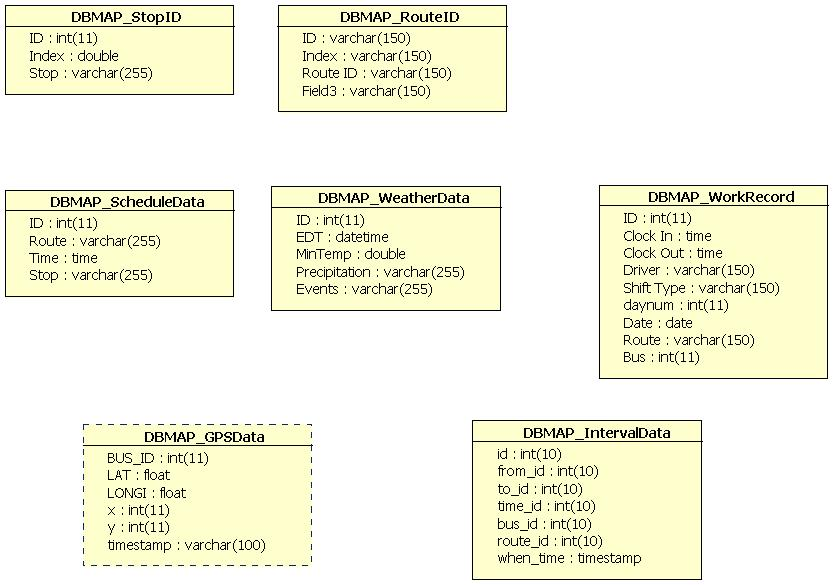
\includegraphics[scale=0.5]{resources/dbmap_access}\\[1cm] 

The tables that are prefixed \lq DBMAP\_\_\rq contain data from DoubleMap. This includes but not limited to schedules, work record (shifts and drivers), Time and Location for each trip for each route with bus that was run in that particular route. \\
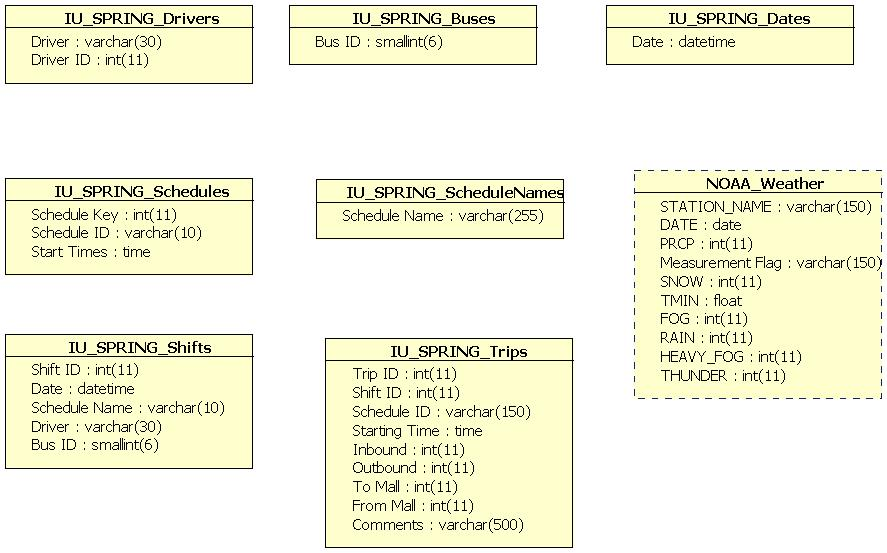
\includegraphics[scale=0.5]{resources/IU_access}\\[1cm] 
The tables that are prefixed \lq IU\_\_\rq contain data maintained by IU Bus System. This included schedules, trips and their overview such as inbound and outbound passenger count. The table prefixed \lq NOAA\_\_\rq was obtained from NOAA\cite{6} for the 
Spring Term 2015\\
\subsection{Base Data Model}
The base tables contain the schedule data from both IU and DBMAP but in the format required to calculate the variation of actual trip time from schedule time. \\
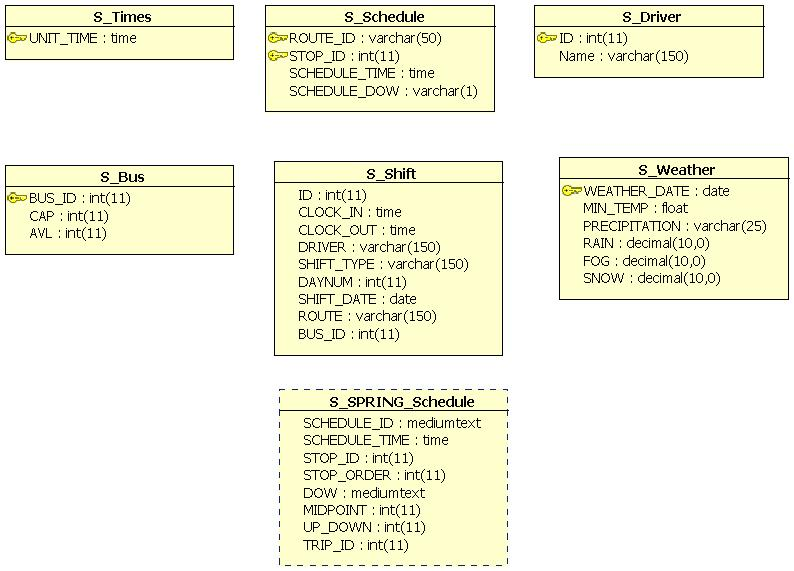
\includegraphics[scale=0.5]{resources/Source_spring}\\[1cm] 

\subsection{Intermediate Model}
Since one of the primary objective was to find how late/early do trips run the tables below are created to be populated with trip/schedule times (The method is explained in next section \lq Data Preparation \rq)\\
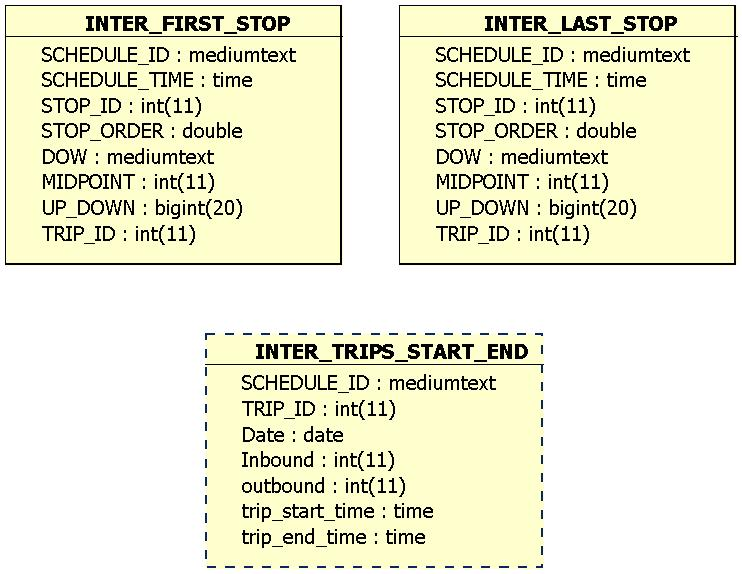
\includegraphics[scale=0.5]{resources/Inter_schedule}\\[1cm] 
The above tables are intermediate tables that are used in calculating \textbf{scheduled} start and end time of each trip\\
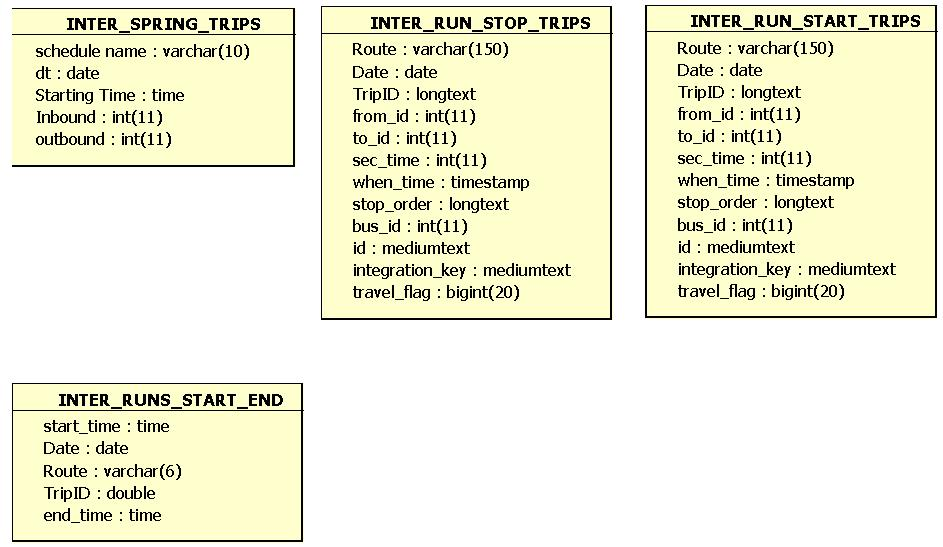
\includegraphics[scale=0.5]{resources/Inter_runs}\\[1cm] 

\subsection{Data Warehouse Model}
The data model by far developed is an OLTP mode	l, which is used for operational efficiency. Inorder to facilitate a better analytic needs, these abstract entities are to be converted to a dimension and fact model. However, instead of traditional OLAP model, we have considered that the dimension to be the schedule and run to be facts. They reside in the model as shown below.\\
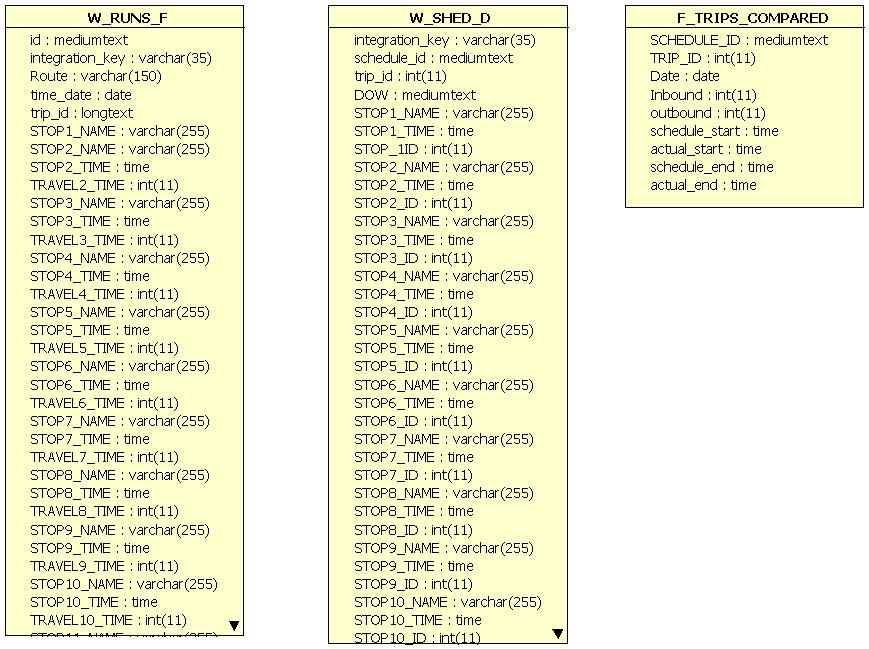
\includegraphics[scale=0.5]{resources/wh}\\[1cm] \\
It can be seen that instead of a one-row per stop approach, this data model now has all trip data in one row. The data model is designed in such a way that it can hold upto 30 stops and a select statement can be used to query the data from these tables and calculate variance.
\subsection{Data Preparation}
This section details the process that was undertaken to convert the data obtained from IU and DBMAP into actionable format. The format of data that is considered actionable is the flattened table format noted in the Data Warehouse model section.
The data preparation involved the following steps:
\begin{enumerate}
\item Generating a TripID for each trip. This is generated by looking at the stop ID and whenever the originating stop occurs, the trip id is incremented.
\item Consolidating different fields such as RouteID, Busid, stopid, time from multiple tables
\end{enumerate}
The above two steps are performed for both schedule data and actual trip data. Now TripId can be further used to compare scheduled and actual time.
As discussed above, the data is now available in OLTP tables with the trip id and stop order. Now asper the data model the data has to be flattened to the new structure.\\
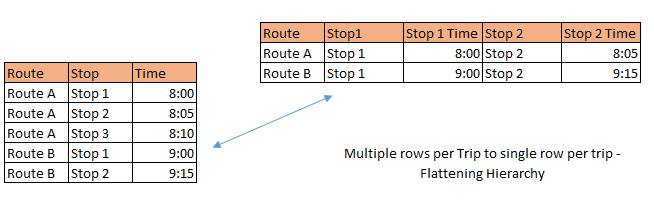
\includegraphics[scale=0.6]{resources/hierarchy}\\[1cm] 
As shown in the above the transformation is made by repeated joins to the same table. For the schedule table,
\begin{verbatim}
concat(DOW,concat('~',concat(trip_id,concat('~',Schedule_ID)))) 'integration_key' 
\end{verbatim}
is used as an integration key. This is nothing but the concatenation of day of week, trip id, and the route if concatenated to create an unique key for every trip. Thus the data is available on the schedule dimension as below,\\
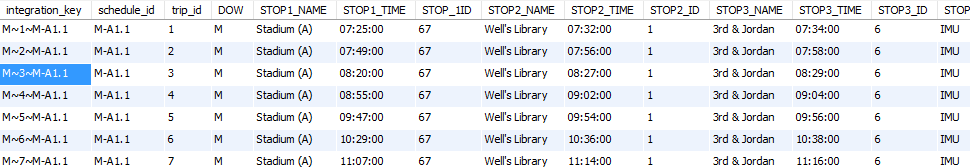
\includegraphics[scale=0.6]{resources/wt1}\\[1cm] 
Once the data to schedule is loaded, now the data to the actual run can be loaded. However to this new table, the unique key is the concatenation of data and the other components as described above. \\
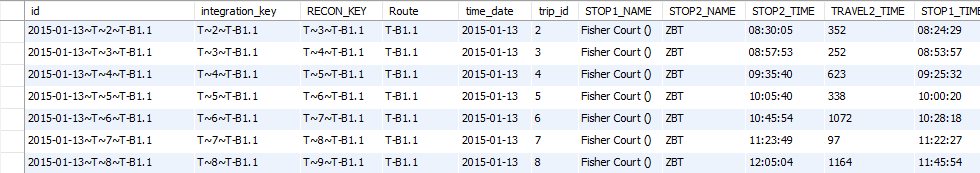
\includegraphics[scale=0.6]{resources/wh2}\\[1cm] 
However, even with this, we would not be able to match the schedule and run. It might happen that for a given trip, the bus may not have stopped in stop 1, hence the whole trip would be lost. Hence we calculate an reconciliation key, $RECON_KEY$. It can be seen that these two keys need not be same and the new key can be used to join with the schedule table to calculate variance. \\
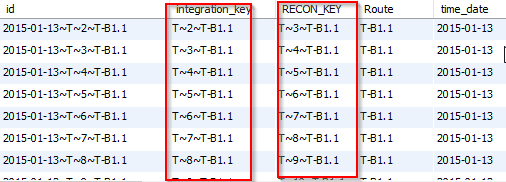
\includegraphics[scale=0.6]{resources/wh3}\\[1cm] 
The variance was just then the select away and is calculated directly.

%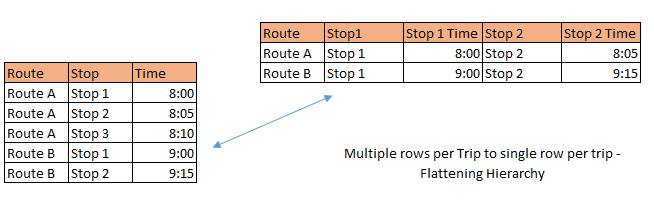
\includegraphics[scale=0.6]{resources/hierarchy}\\[1cm] 

\section{Exploratory Analysis}
Any Start of Data Analytics involves understanding of the data. An initial Exploratory data analysis was made using R and ggplot2 library. For example the below graph indicates the average time between the pairs of stops for the 12 AM for Route A. It can be seen that the travelling time is very less during morning 12AM. \\
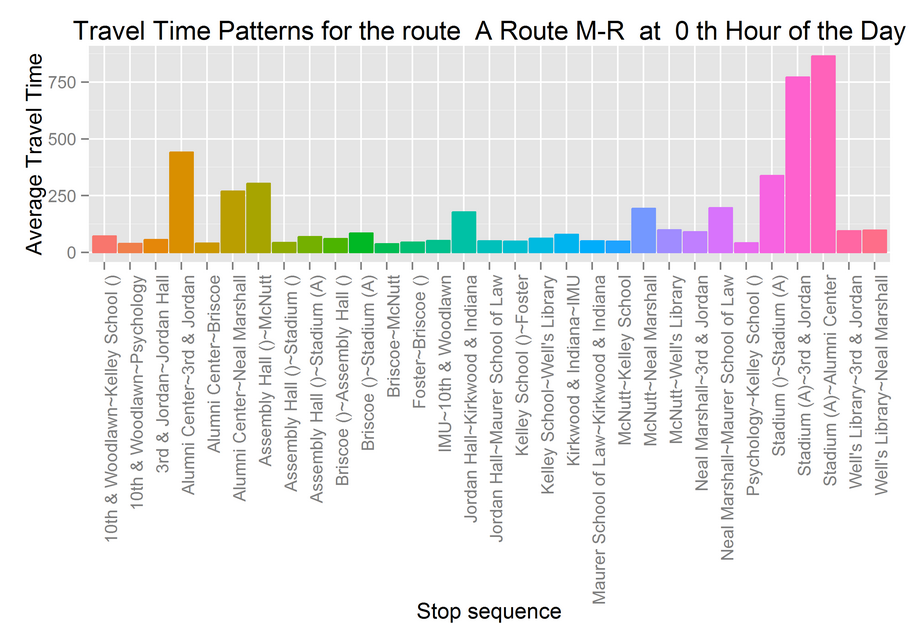
\includegraphics[scale=0.4]{resources/ggplot1}\\[1cm] 
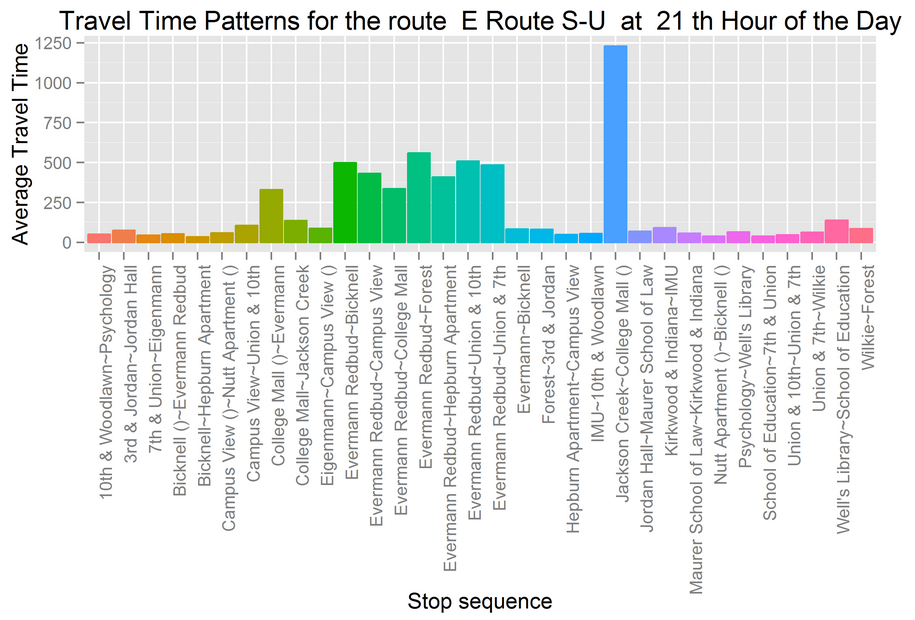
\includegraphics[scale=0.4]{resources/ggplot2}\\[1cm] 
However, a change in trend happens during the "peak times". During evening 7, the average time traveling time increases drastically, for Eg, 10th and Wood Lawn to psychology takes less than a minute during morning, however during evenings, it double to about 2 minutes. The same trend can be seen at below plots. \\
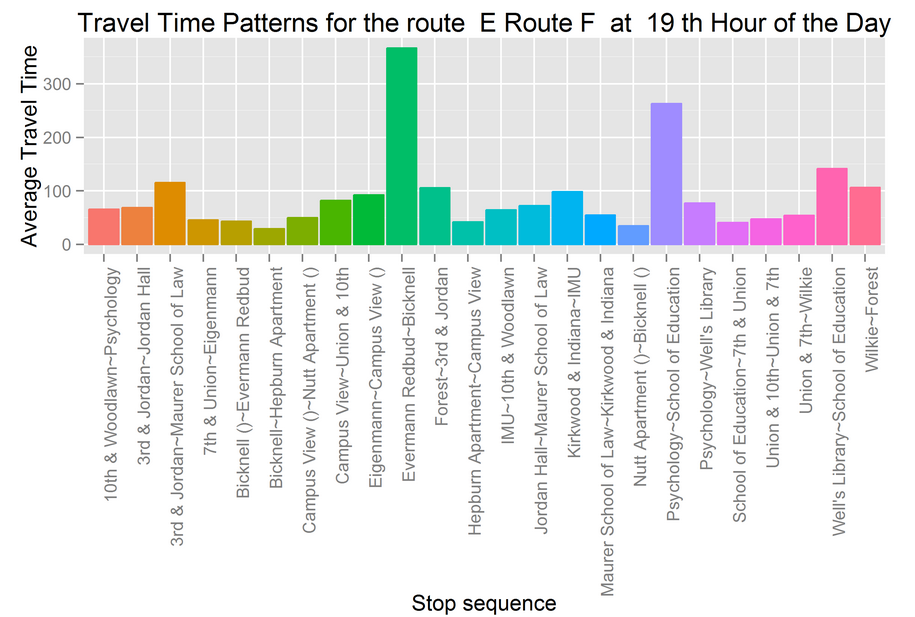
\includegraphics[scale=0.4]{resources/ggplot3}\\[1cm] 
However things get different when we talk about the dwell time. The average dwell time was plotted for every single hour of the day, it is interesting to note that the maximum time the bus spends is in the originating stops! \\
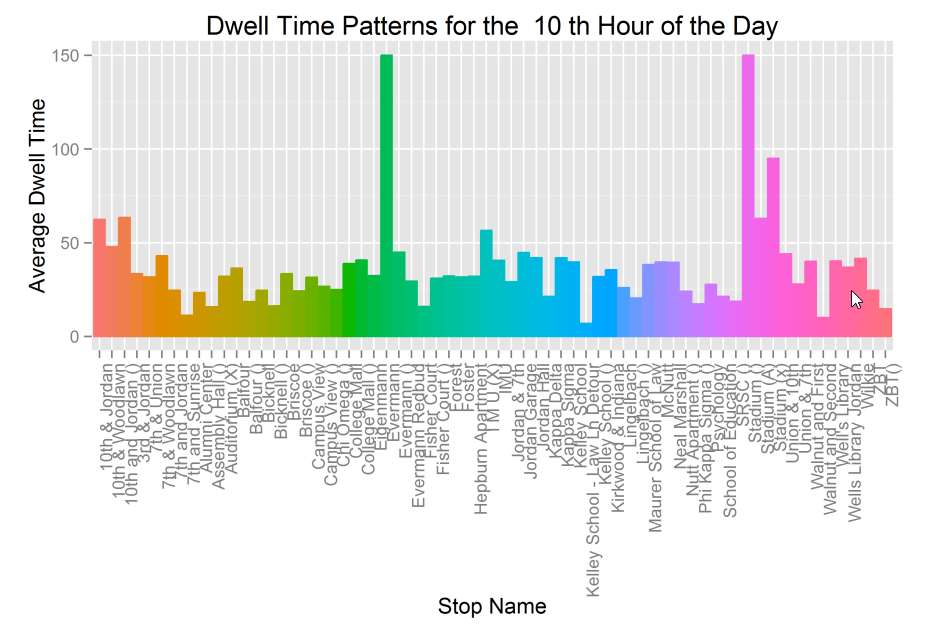
\includegraphics[scale=0.4]{resources/ggplot4}\\[1cm] 
Another interesting trend is that as the day progresses, dwell time increases in major stops. There is in fact spike in the major stops like IMU, Kirkwood and Indiana and Kelley's school of Business. \\
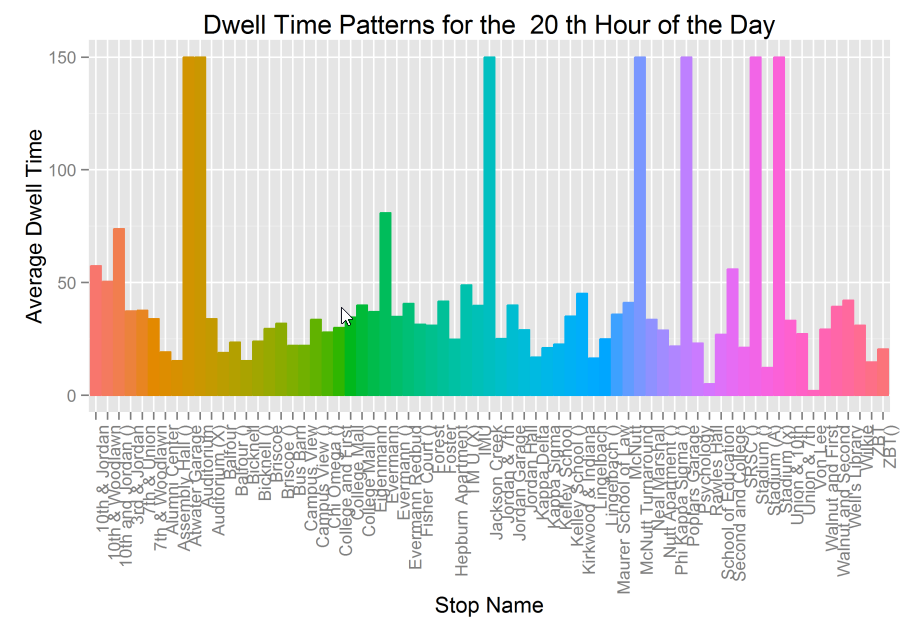
\includegraphics[scale=0.4]{resources/ggplot5}\\[1cm] 
All these graphs and more visualizations are available in the Github Repository, \url{https://github.com/sarvothaman/nefarious-octo-rutabaga/tree/master/EDA}
\section{Reporting}
The Main objective of this case study is to report how much the busses run in accordance to the schedule. ie, the time deviation $t_{schedule}-t_{acutal}$ is an important metric. Tableau reporting solution was used to report these findings. \\
Tableau provides an excellent platform for developing these reports. The variance reports are reports which gives the flexibility to select the month, data, route and trip and check the variance in each stops. This is available on cloud and can be accessed by anyone for free. Below is the screenshot of the application hosted.\\
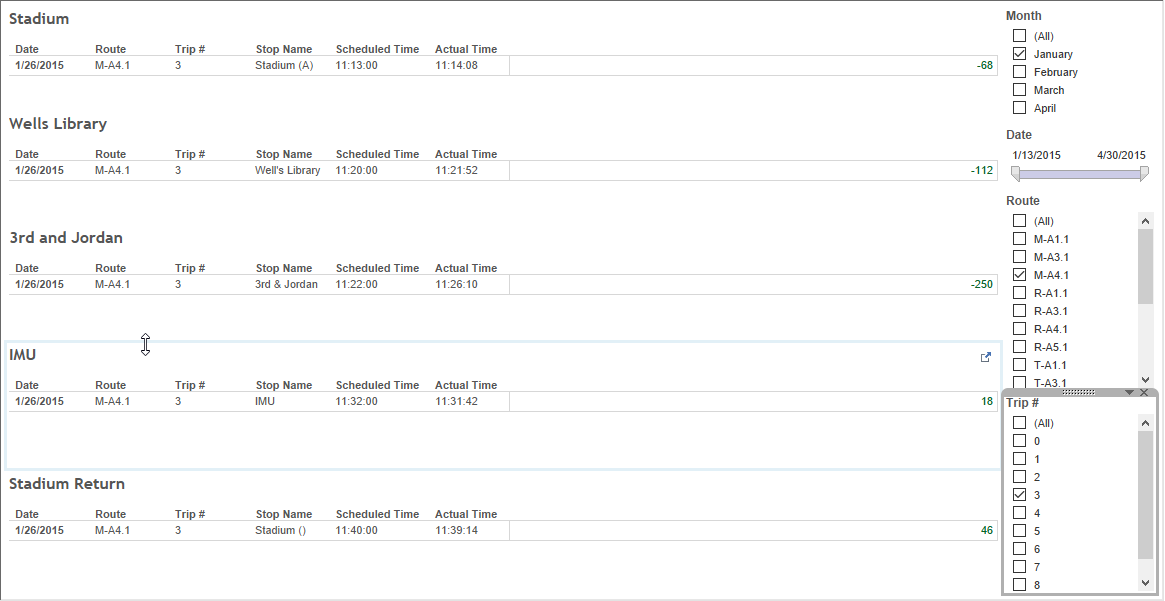
\includegraphics[scale=0.4]{resources/tableau4}\\[1cm] 
For example, the above shown trip is the 3 trip of A1 on January 26th 2015. It can be seen that the departure from stadium A is at 11:13, however the bus departed at 11:14 bringing in an one minute delay. It is interesting that in 3rd and Jordan, the was about 3 minutes late, however it reached IMU one minute early. This suggests that there is still space for optimizing the schedule. Multiple trips can also be selected as shown below to access trip information.
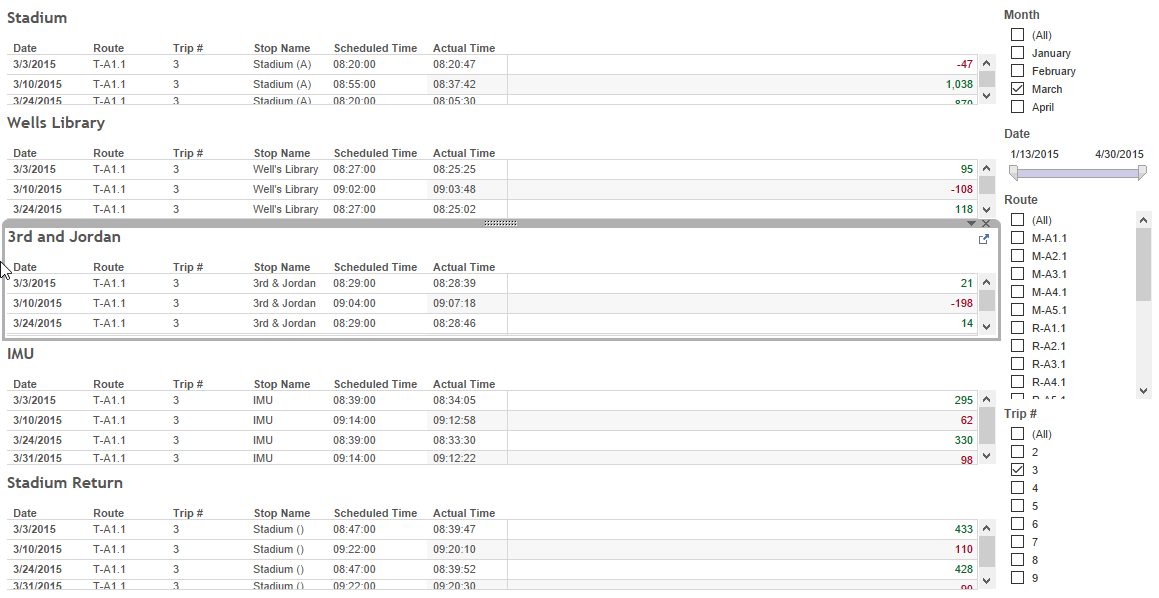
\includegraphics[scale=0.4]{resources/tableau5}\\[1cm] 
\textbf{Status Reports}\\
Sometimes we are interested in seeing that only whether the bus has arrived on-time or early to the main stops. The below report is called the logistic report and is available on cloud. This gives the user the option to drill down a specific date, month, route then trip and displays the status.\\
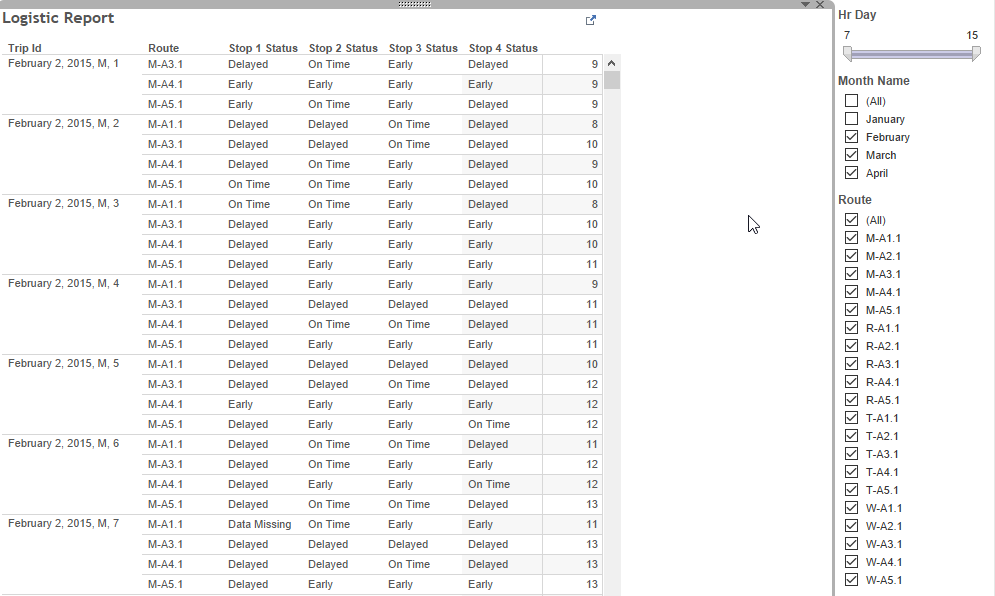
\includegraphics[scale=0.5]{resources/tableau6}\\[1cm] 
For example the Feburary 2nd, A4 route, 1st trip reached all its stop ahead time.\\
Thus care has been taken during this case study that due importance is given to usability of the output artifacts and can be used by the business rather than the esoteric data miners.
\section{Visualization}
Another aspect of the data is the ability to visualize the data to understand the route. Neo4j is used as the background data store for saving node data. pyMysql module was used to connect to mysql and py2neo was used to connect to the cloud instance.\\
A python program was written to aggregate the data from MySql and load it to cloud Neo4j instance. Once the entire data is loaded, the graph looks as follows.\\
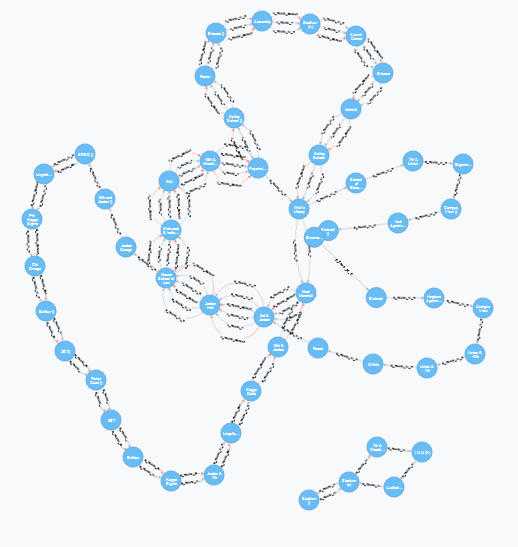
\includegraphics[scale=0.8]{resources/neo4j1}\\[1cm] 
A close in screenshot is as follows. The data model is created in such a way that each stops are represented as nodes and each directed arrow is the route. These edges has a properties like travel time at any given hour of the day and the nodes contain average dwell time in that stop for a given day\\
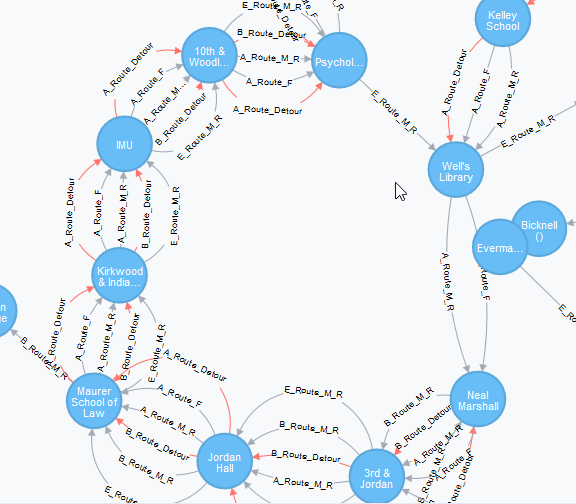
\includegraphics[scale=0.8]{resources/neo4j2}\\[1cm] 
Neo4j uses the language called Cypher instead of the SQL query. An example cypher query is as follows\\
\begin{verbatim}
MATCH p =(a:Stops { name: "Neal Marshall" })
-[:A_Route_M_R *]-
(b:Stops { name: "IMU" })
RETURN p, length(p)
\end{verbatim}
The above cypher selects a path from Neal Marshall to IMU and follows the route A in the Monday to Thursday schedule.\\
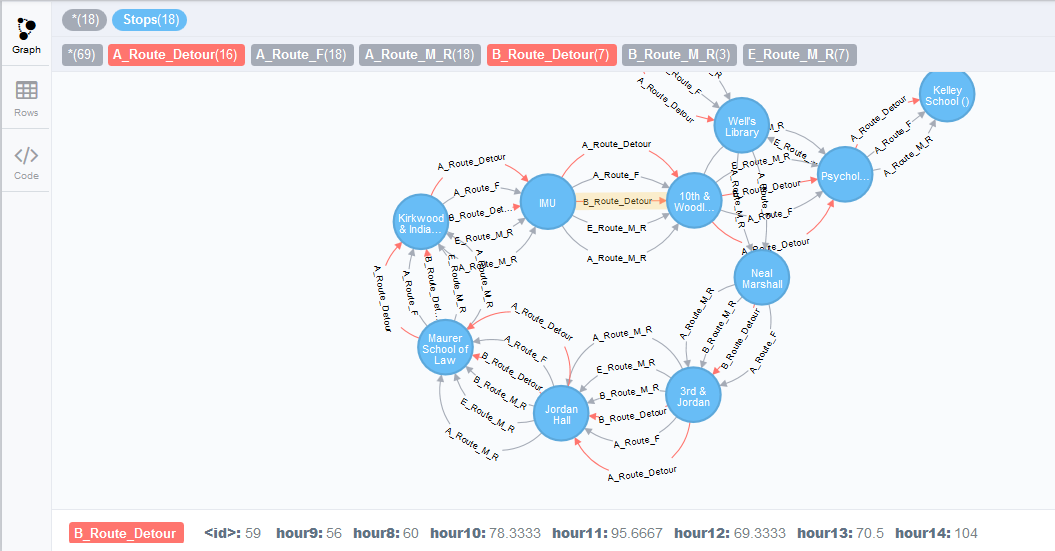
\includegraphics[scale=0.45]{resources/neo4j3}\\[1cm] 
It can be seen below that there are parameters like hour9 indicates the travelling time at 9th hour of the day. This was used to predict the delay/arrival time and most of the time it predicted the time accurate upto Plus or minus three minutes.\\ \\
\textbf{Status Reporting} \\
As seen in above reports, for effective decision making the counts of instances bus statuses over a period of time is important. The below plots help in such interpretation,\\
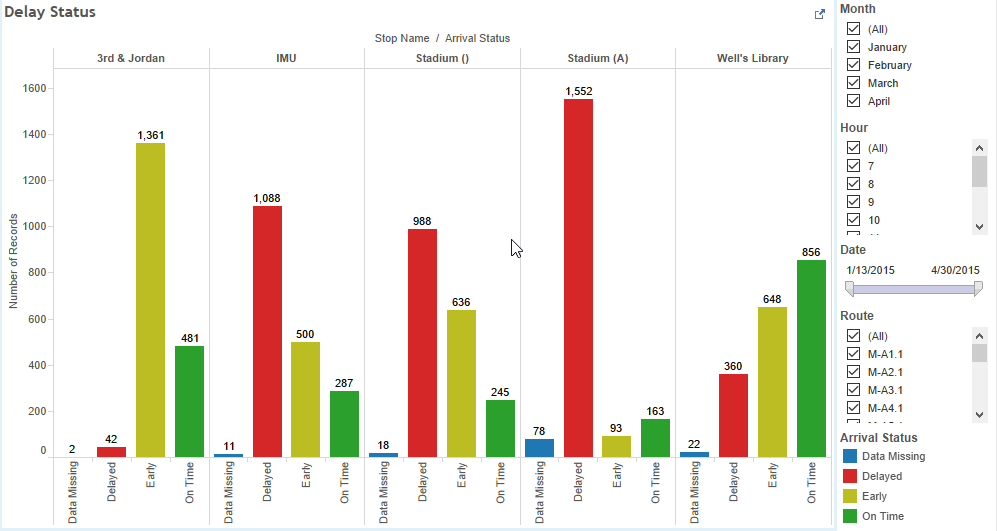
\includegraphics[scale=0.55]{resources/tableau1}\\[1cm] 
Eg, the above graph gives the count of the instances of the statuses. Generally it can be seen that stadium is always delayed and wells library is always on time.\\
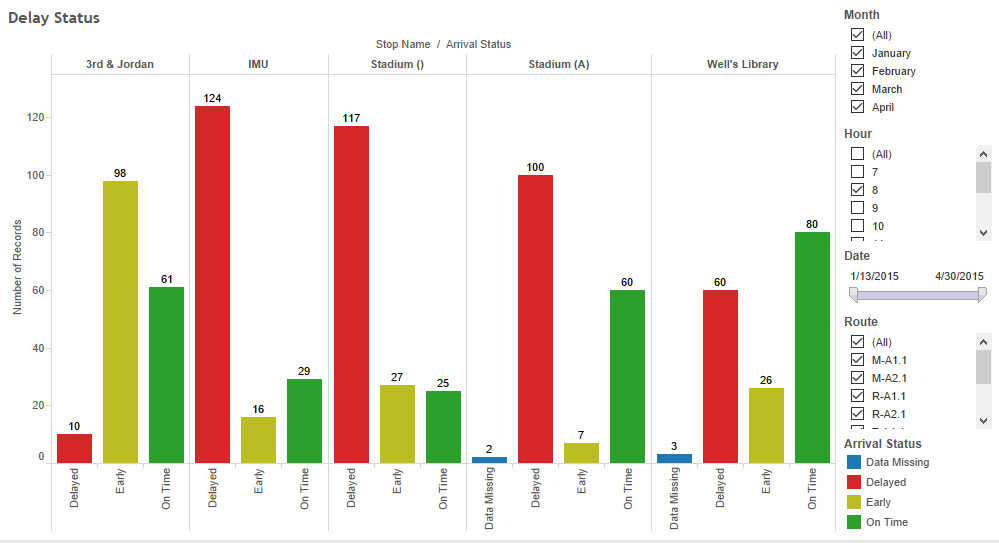
\includegraphics[scale=0.55]{resources/tableau2}\\[1cm] 
This also lets the user to select the hour of the day, month, day, route and see how the delay status is affected.\\
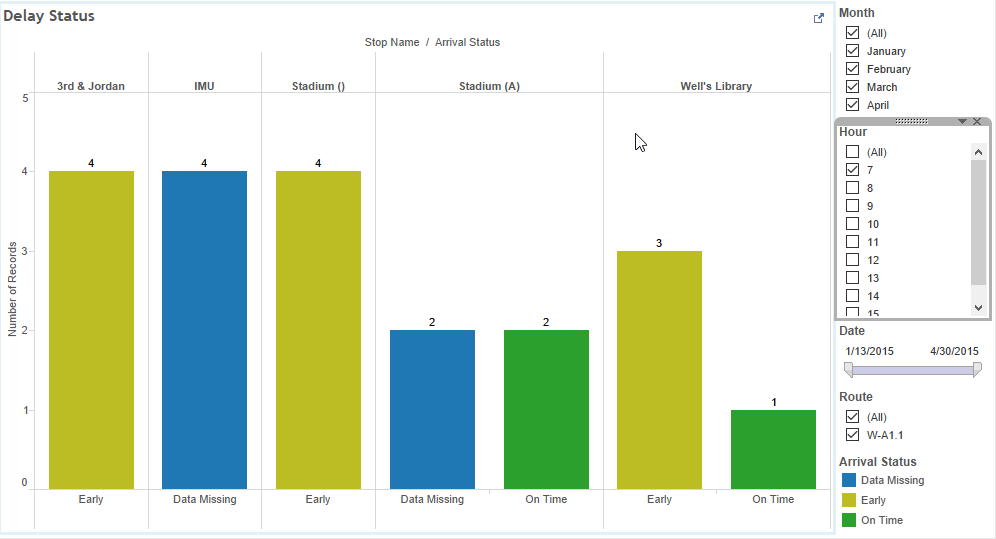
\includegraphics[scale=0.55]{resources/tableau3}\\[1cm] 
In refreshing change, During the mornings, for most of the stops the bus reaches either early or on time.
\section{Statistical Model}
\textbf{Logistic Regression Model}

The data from the MySql database was made longitudinal again and was exported as an CSV file. This file as sourced to the R.\\

A logistic Regression model was built over this dataset to predict whether the thr A Route would be On-Time, or Delayed or Early.\\

As described earlier, if the actual time is a minute or earlier than the schedule time, it is marked Early. If the bus arrives a minute before or after the scheduled time, then it is termed as On-Time. If the bus is delayed by more than a minute, it is termed as late.\\

In essense,\\
On time : one min before and after the scheduled time\\
Early: Earlier than a minute to the scheduled time\\
Late: Later than a minute to the scheduled time\\

Thus, the logistic model would have 3 levels, On-Time, Early and Delayed.\\

**Model 1** The model was built in such a way that the prediction in first stop would dependant on the tie of the hour and the trip of the day.\\
**Model 2** The second model was built in such a way that this would consider the status of arrival in the first stop, hour and the day of travel.\\
**Iterative Models** The consecutive models for stops iteratively built on this process, all constant factors and the previous stop status
\begin{knitrout}
\definecolor{shadecolor}{rgb}{0.969, 0.969, 0.969}\color{fgcolor}\begin{kframe}
\begin{alltt}
\hlkwd{setwd}\hlstd{(}\hlstr{"C:\textbackslash{}\textbackslash{}Users\textbackslash{}\textbackslash{}Sarvo\textbackslash{}\textbackslash{}nefarious-octo-rutabaga\textbackslash{}\textbackslash{}R Models\textbackslash{}\textbackslash{}Data"}\hlstd{)}
\hlkwd{library}\hlstd{(nnet)}
\hlstd{routea}\hlkwb{<-}\hlkwd{read.csv}\hlstd{(}\hlstr{"DATA.csv"}\hlstd{)}
\hlcom{# Stop 1 Model}
\hlstd{stop1.fit}\hlkwb{<-}\hlkwd{multinom}\hlstd{(Stop.1.Status}\hlopt{~}\hlstd{Day}\hlopt{+}\hlstd{Hr.Day,}\hlkwc{data}\hlstd{=routea)}
\end{alltt}
\begin{verbatim}
## # weights:  24 (15 variable)
## initial  value 2614.551165 
## iter  10 value 1136.297534
## iter  20 value 1087.220212
## final  value 1087.212606 
## converged
\end{verbatim}
\begin{alltt}
\hlcom{# Predict Stop 1 Status}
\hlstd{stop1.prob}\hlkwb{<-}\hlkwd{data.frame}\hlstd{(}\hlkwc{Day}\hlstd{=}\hlkwd{c}\hlstd{(}\hlstr{"M"}\hlstd{),}\hlkwc{Hr.Day}\hlstd{=}\hlnum{10}\hlstd{)}
\hlkwd{predict}\hlstd{(stop1.fit,}\hlkwc{newdata} \hlstd{= stop1.prob,}\hlstr{"probs"}\hlstd{)}
\end{alltt}
\begin{verbatim}
## Data Missing      Delayed        Early      On Time 
##   0.03082123   0.77910313   0.07317609   0.11689955
\end{verbatim}
\begin{alltt}
\hlcom{#Stop 2 status}
\hlstd{stop2.fit}\hlkwb{<-}\hlkwd{multinom}\hlstd{(Stop.2.Status}\hlopt{~}\hlstd{Day}\hlopt{+}\hlstd{Hr.Day}\hlopt{+}\hlstd{Stop.1.Status,}\hlkwc{data}\hlstd{=routea)}
\end{alltt}
\begin{verbatim}
## # weights:  36 (24 variable)
## initial  value 2614.551165 
## iter  10 value 2117.757741
## iter  20 value 2011.097163
## iter  30 value 1998.078206
## iter  40 value 1997.885031
## final  value 1997.884320 
## converged
\end{verbatim}
\begin{alltt}
\hlcom{#Prediction for Stop 2 status}
\hlstd{stop2.prob}\hlkwb{<-}\hlkwd{data.frame}\hlstd{(}\hlkwc{Day}\hlstd{=}\hlkwd{c}\hlstd{(}\hlstr{"M"}\hlstd{),}\hlkwc{Hr.Day}\hlstd{=}\hlnum{10}\hlstd{,}\hlkwc{Stop.1.Status}\hlstd{=}\hlkwd{c}\hlstd{(}\hlstr{"Delayed"}\hlstd{))}
\hlkwd{predict}\hlstd{(stop2.fit,}\hlkwc{newdata} \hlstd{= stop2.prob,}\hlstr{"probs"}\hlstd{)}
\end{alltt}
\begin{verbatim}
## Data Missing      Delayed        Early      On Time 
##   0.01664346   0.14224930   0.36711064   0.47399660
\end{verbatim}
\begin{alltt}
\hlcom{#Stop 3 Status}
\hlstd{stop3.fit}\hlkwb{<-}\hlkwd{multinom}\hlstd{(Stop.3.Status}\hlopt{~}\hlstd{Day}\hlopt{+}
                                                \hlstd{Hr.Day}\hlopt{+}
                                                \hlstd{Stop.1.Status}\hlopt{+}
                                                \hlstd{Stop.2.Status,}
                                        \hlkwc{data}\hlstd{=routea)}
\end{alltt}
\begin{verbatim}
## # weights:  48 (33 variable)
## initial  value 2614.551165 
## iter  10 value 861.842048
## iter  20 value 708.720592
## iter  30 value 685.807742
## iter  40 value 684.351992
## iter  50 value 684.315511
## final  value 684.313809 
## converged
\end{verbatim}
\begin{alltt}
\hlcom{#Prediction for Stop 3}
\hlstd{stop3.prob}\hlkwb{<-}\hlkwd{data.frame}\hlstd{(}\hlkwc{Day}\hlstd{=}\hlkwd{c}\hlstd{(}\hlstr{"M"}\hlstd{),}\hlkwc{Hr.Day}\hlstd{=}\hlnum{10}\hlstd{,}
                                           \hlkwc{Stop.1.Status}\hlstd{=}\hlkwd{c}\hlstd{(}\hlstr{"Delayed"}\hlstd{),}
                                           \hlkwc{Stop.2.Status}\hlstd{=}\hlkwd{c}\hlstd{(}\hlstr{"On Time"}\hlstd{))}
\hlkwd{predict}\hlstd{(stop3.fit,}\hlkwc{newdata} \hlstd{= stop3.prob,}\hlstr{"probs"}\hlstd{)}
\end{alltt}
\begin{verbatim}
## Data Missing      Delayed        Early      On Time 
## 3.381334e-03 7.365777e-11 7.682267e-01 2.283920e-01
\end{verbatim}
\begin{alltt}
\hlcom{# Stop 4 Model}
\hlstd{stop4.fit}\hlkwb{<-}\hlkwd{multinom}\hlstd{(Stop.4.Status}\hlopt{~}\hlstd{Day}\hlopt{+}
                                                \hlstd{Hr.Day}\hlopt{+}
                                                \hlstd{Stop.1.Status}\hlopt{+}
                                                \hlstd{Stop.2.Status}\hlopt{+}
                                                \hlstd{Stop.3.Status,}
                                        \hlkwc{data}\hlstd{=routea)}
\end{alltt}
\begin{verbatim}
## # weights:  60 (42 variable)
## initial  value 2614.551165 
## iter  10 value 1261.966796
## iter  20 value 1136.788612
## iter  30 value 1099.663056
## iter  40 value 1096.691497
## iter  50 value 1096.544668
## iter  60 value 1096.531568
## final  value 1096.531328 
## converged
\end{verbatim}
\begin{alltt}
\hlcom{#Prediction}
\hlstd{stop4.prob}\hlkwb{<-}\hlkwd{data.frame}\hlstd{(}\hlkwc{Day}\hlstd{=}\hlkwd{c}\hlstd{(}\hlstr{"M"}\hlstd{),}
                                           \hlkwc{Hr.Day}\hlstd{=}\hlnum{10}\hlstd{,}
                                           \hlkwc{Stop.1.Status}\hlstd{=}\hlkwd{c}\hlstd{(}\hlstr{"Delayed"}\hlstd{),}
                                           \hlkwc{Stop.2.Status}\hlstd{=}\hlkwd{c}\hlstd{(}\hlstr{"On Time"}\hlstd{),}
                                           \hlkwc{Stop.3.Status}\hlstd{=}\hlkwd{c}\hlstd{(}\hlstr{"On Time"}\hlstd{))}
\hlkwd{predict}\hlstd{(stop4.fit,}\hlkwc{newdata} \hlstd{= stop4.prob,}\hlstr{"probs"}\hlstd{)}
\end{alltt}
\begin{verbatim}
## Data Missing      Delayed        Early      On Time 
## 2.966553e-18 9.588480e-01 8.424239e-12 4.115202e-02
\end{verbatim}
\end{kframe}
\end{knitrout}
A keen observer can see that this prediction is as same as the results off Tableau Graphs. Even there, the pattern that was observed is that if the bus starts delayed, it comes on-time to Stop 2, and comes Delayed to Stop 3.\\

Thus this model can give a cateogorical answers to queries about the existing status of the bus.\\

\section{Concluding remarks}
Throughout our exploratory analysis and modeling we were able to make observations that are consistent with reality (verified by logic as well as with actual data) as well as make certain predictions (using neo4j model for example). While the results are preliminary and simple in nature, the framework and methods of analysis can be easily extended. We consider this an important step, since ability to quicky analyze the data is critical in achieving the overall objectives
\section{Future Work}

\section{References}
\bibliographystyle{unsrt} 
	\bibliography{ref}
\end{document}
